\scanpage{171}
% archive sheet number: 170
% Four long diagonal cancellation strokes cross the working sheet.
\deleted{$X_1\qquad X_2$}
\diagram{\begin{tikzcd}[ampersand replacement=\&,column sep=small]
\deleted{X'''} \arrow[d,shift left=1.4pt,no head] \arrow[d,no head] \arrow[d,shift right=1.4pt,no head] \& \deleted{\pi_0(X''')} \\
\deleted{X''} \arrow[d,shift left=.8pt,no head] \arrow[d,shift right=.8pt,no head] \& \deleted{\pi_0(X'')} \\
\deleted{X'} \arrow[d,no head] \& \deleted{\pi_0(X')}\quad\text{\deleted{\uline{un seul pt}}} \\
\deleted{X} \&
\end{tikzcd}}

\diagram{\begin{tikzcd}[ampersand replacement=\&]
\deleted{\pi_1(X',\bar x)} \arrow[d] \\
\deleted{\pi_1(X,\bar x)}
\end{tikzcd}}
\deleted{$P\subset I$ \unsure{opère} \unsure{triv\textsuperscript{t}|trivialm.} sur $\pi_1(X',\bar x)$ donc sur son \unsure{image}.}

\figure{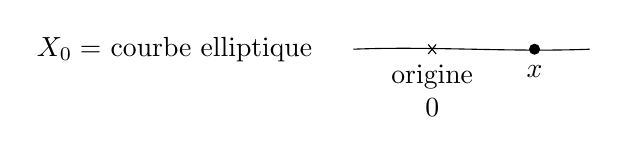
\begin{tikzpicture}
\node[anchor=east] at (-.4,0) {\deleted{$X_0=$ courbe elliptique}};
\draw (0,0) .. controls (1,.04) and (2,-.04) .. (3,0);
\draw (.95,-.06)--(1.05,.06) (.95,.06)--(1.05,-.06);
\fill (2.3,0) circle (2pt);
\node[below,align=center] at (1,-.08) {\deleted{origine}\\\deleted{$0$}};
\node[below] at (2.3,-.08) {\deleted{$x$}};
\end{tikzpicture}}
\figure{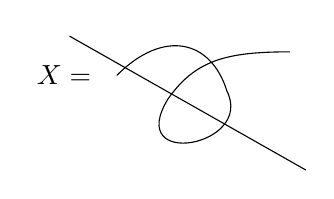
\begin{tikzpicture}
\node[anchor=east] at (-.2,0) {\deleted{$X=$}};
\draw (0,0) .. controls (.6,.6) and (1.2,.45) .. (1.4,-.2)
.. controls (1.75,-.9) and (.1,-1.2) .. (.65,-.3)
.. controls (1,.2) and (1.4,.3) .. (2.2,.3);
\draw (-.6,.5)--(2.4,-1.2);
\end{tikzpicture}}
\[
\deleted{H^0(K,A)\longrightarrow H^1(K,T_\ell(A))}
\]

\diagram{\begin{tikzcd}[ampersand replacement=\&,column sep=small,row sep=large]
\deleted{X} \arrow[dd] \& \deleted{X_K} \arrow[l] \arrow[dd] \& \& \deleted{X_{\unsure{\widetilde U|\widetilde\eta}}} \arrow[ll] \arrow[dd,no head] \& \\
\& \& \deleted{X} \arrow[ul] \arrow[dd,no head] \& \& \deleted{\widetilde X} \arrow[ul] \arrow[ll] \arrow[dd,no head] \quad \deleted{\unsure{F_{\bar a}|F_{\bar\alpha}}} \\
\deleted{S} \arrow[uu,bend left=20] \& \deleted{U} \arrow[l,hook'] \arrow[uu,bend left=20] \& \& \deleted{\bar U} \arrow[ll] \& \\
\& \& \deleted{S} \arrow[ul] \& \& \deleted{\bar S} \arrow[ll] \arrow[ul]
\end{tikzcd}}

\diagram{\begin{tikzcd}[ampersand replacement=\&]
\deleted{\unsure{\mathscr B|B}_{\unsure{\Gamma|\mathscr T|T}}} \arrow[d] \& \deleted{\mathscr B_\pi} \arrow[l] \arrow[d] \& \\
\deleted{\unsure{P|p}} \& \deleted{\mathscr B_I} \arrow[l] \& \deleted{P} \arrow[l]
\end{tikzcd}}
